\subsection{RQ1: Where does planning beat direct execution?}
\label{sec:rq1}
\begin{figure*}[!t]
\centering
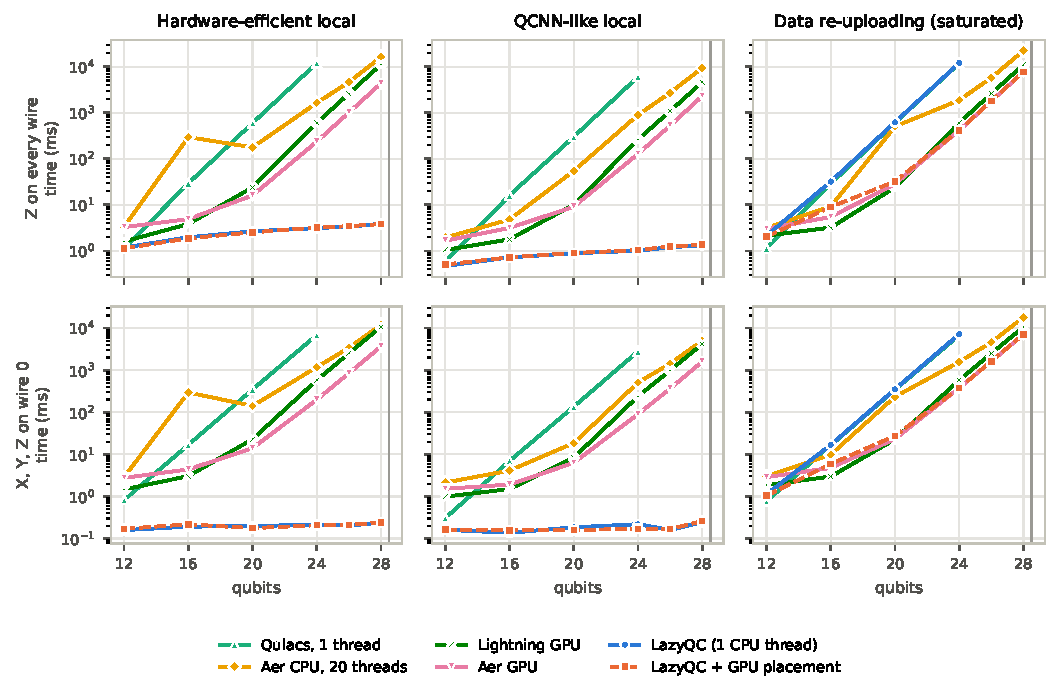
\includegraphics[width=\textwidth]{figures/direct_scaling.pdf}
\caption{Time to obtain every requested expectation value as the register grows, for the three circuit families (columns) and the two output patterns (rows). Each point is the median over repetitions of one case, averaged geometrically over two held-out seeds. The planner runs on one CPU thread and is charged with its analysis; direct methods receive prebuilt circuits and all 20 host threads. The vertical line marks the 28-qubit limit of the 8\,GB GPU in double precision. Aer CPU is slower at 16 than at 20 qubits on the hardware-efficient family, where synchronizing 20 threads dominates the small state. Lower is better.}
\label{fig:direct-scaling}
\end{figure*}

\begin{table}[!t]
\caption{Fastest Direct Method's Time Divided by the Planner's Time, with GPU Placement Enabled, by Number of Qubits. Values Above One Favour the Planner.}
\label{tab:rq1}
\centering
\setlength{\tabcolsep}{3pt}
\footnotesize
\resizebox{\columnwidth}{!}{\begin{tabular}{llrrrrrr}
\toprule
Family & Outputs & 12 & 16 & 20 & 24 & 26 & 28\\
\midrule
Hardware-eff. & $Z$, all & 1.00 & 2.05 & 6.34 & 73.3 & 295 & 1{,}137\\
Hardware-eff. & $X,Y,Z$, one & 4.84 & 14.0 & 79.5 & 960 & 3{,}987 & 15{,}279\\
QCNN-like & $Z$, all & 1.15 & 2.46 & 10.2 & 122 & 424 & 1{,}681\\
QCNN-like & $X,Y,Z$, one & 1.87 & 9.55 & 39.6 & 529 & 2{,}177 & 6{,}111\\
Re-uploading & $Z$, all & 0.56 & 0.36 & 0.74 & 1.00 & 1.00 & 1.00\\
Re-uploading & $X,Y,Z$, one & 0.74 & 0.50 & 0.83 & 1.01 & 1.00 & 1.00\\
\bottomrule
\end{tabular}
}
\end{table}

Fig.~\ref{fig:direct-scaling} shows the time needed to obtain every requested output as the register grows from 12 to 28 qubits, and Table~\ref{tab:rq1} gives the ratio between the fastest direct method and the planner. Three regimes stand out.

\textbf{Local families: work that no device can avoid.} For the hardware-efficient and QCNN-like families, the planner's time is almost flat. With $Z$ on every wire, it grows from 1.1 to 3.8\,ms (hardware-efficient) and from 0.5 to 1.4\,ms (QCNN-like) between 12 and 28 qubits, because every output keeps a cone of at most 10 and 8 qubits respectively, while every direct method doubles its cost with each added qubit. At 28 qubits the planner groups the 28 outputs of the hardware-efficient circuit into 14 tasks of at most 10 qubits and spends 1.4\,ms planning and 2.3\,ms collecting them, whereas the fastest direct method, Aer on the GPU, needs 4.35\,s. On a single CPU thread the planner ties with single-thread Qulacs at 12 qubits, and is 2.0 to 2.5 times faster than the fastest GPU method at 16 qubits (1.6 to 2.2 times in a later confirmation run), 6 to 10 times at 20, 73 to 122 times at 24 and 1,137 to 1,681 times at 28. When only the three Paulis on one wire are requested, a dense state serves fewer outputs and the margins grow further, from 1.9 to 4.8 times at 12 qubits to 6,111 to 15,279 times at 28. These ratios are large because the direct curves grow exponentially while the planner's do not. They are specific to our laptop GPU, but a faster GPU moves the direct curves down by a constant factor without changing their slope (Section~\ref{sec:discussion}).

\textbf{Saturated cones: hand the work over.} In the data re-uploading family every cone spans the whole register and the planner keeps the dense plan. On one CPU thread this costs what single-thread Qulacs costs plus the planner's overhead, which is visible at small widths (2.1 against 1.1\,ms at 12 qubits) and negligible at large ones (12.1 against 11.9\,s at 24 qubits). With width-based placement the dense task runs on the GPU instead. The fixed costs of planning, lowering the circuit and launching it make the planner 0.36 to 0.83 times as fast as the fastest GPU method between 16 and 20 qubits, but from 24 qubits on it matches direct Aer GPU within 0.6\% (0.997 to 1.006 times). The planner cannot speed up saturated work, but it does not need to make it slower either.

\textbf{Small circuits.} At 12 qubits every method takes about a millisecond and fixed costs dominate the comparison. The planner pays up to 0.6\,ms of analysis and 0.4\,ms of circuit lowering that direct methods with prebuilt circuits do not pay. It is still 1.15 to 4.8 times faster than the best direct method on three of the four local configurations, ties on the fourth and is 0.56 to 0.74 times as fast on the saturated control. The analysis budget of Section~\ref{sec:system} only skips analysis that could not pay even if every cone were free, so it rarely triggers at these sizes; RQ3 examines its effect on the cost of deciding.

\begin{table}[!t]
\caption{Held-Out Families on One CPU Thread: Planner Time over Direct Qulacs and Cross-Validated Selection Regret, Medians per Stratum at One Collection. The Five Top Strata Are Disjoint and Sum to 480; the Width Rows Break Down Their 405-Case Saturated Subset and Are Not Added Again. F, S and G Count the Full, Separate and Grouped Plans Chosen by \texttt{auto}.}
\label{tab:heldout}
\centering
\setlength{\tabcolsep}{3pt}
\footnotesize
\resizebox{\columnwidth}{!}{\begin{tabular}{lrlrr}
\toprule
Stratum & Cases & Auto choice & Auto/direct & CV regret\\
\midrule
\multicolumn{5}{l}{\emph{Disjoint family/cone strata (480 cases)}}\\
Tree, narrow, shared & 15 & G\,15 & 0.016 & 1.14\\
Tree, narrow, distinct & 10 & S\,10 & 0.003 & 1.07\\
Tree, intermediate & 50 & S\,35, G\,15 & 0.29 & 1.05\\
Tree, saturated & 165 & F\,100, G\,55, S\,10 & 1.12 & 1.06\\
Strongly ent., saturated & 240 & F\,170, G\,70 & 1.07 & 1.04\\
\midrule
\multicolumn{5}{l}{\emph{Width breakdown of the 405 saturated cases (overlapping rows)}}\\
Saturated, 8 qubits & 105 & F\,75, G\,30 & 1.82 & 1.41\\
Saturated, 12 qubits & 105 & F\,70, G\,35 & 1.24 & 1.13\\
Saturated, 16 qubits & 105 & F\,70, G\,30, S\,5 & 1.04 & 1.03\\
Saturated, 20 qubits & 90 & F\,55, G\,30, S\,5 & 1.00 & 1.00\\
\midrule
\multicolumn{5}{l}{\emph{All 480 cases (each counted once)}}\\
All held-out cases & 480 & F\,270, G\,155, S\,55 & 1.07 & 1.05\\
\bottomrule
\end{tabular}
}
\end{table}

\textbf{Unseen families.} The same regimes appear on the two families added after the planner was frozen (Table~\ref{tab:heldout}), here against direct single-thread Qulacs at depths 2 to 16. Where tree cones are narrow and outputs share them, the planner needs 0.016 times the direct time, about 60 times less. With narrow cones that outputs do not share it needs 0.003 times, and with intermediate cones 0.29 times. Where cones saturate, \texttt{auto} keeps the dense plan in two thirds of the cases and pays 1.07 to 1.12 times direct execution. That overhead is a matter of size rather than family: 1.82 times at 8 qubits, where a direct evolution takes 0.2\,ms, 1.24 at 12, 1.04 at 16 and 1.00 at 20. The fixed cost of deciding is visible only while the simulation itself takes about a millisecond.

\begin{table}[!t]
\caption{Same-Backend Comparison with $Z$ on Every Wire: Direct Execution Time Divided by the Time of LazyQC Running Its Tasks on the Same Backend, by Number of Qubits. Values Above One Favour LazyQC. Qulacs Uses One Thread; LazyQC on quimb Uses the Grouped Cone Plan. The quimb Row Is the Legacy Per-Output Comparator; Stronger Shared Tensor-Network Baselines Appear Below.}
\label{tab:backends}
\centering
\setlength{\tabcolsep}{3pt}
\footnotesize
\begin{tabular}{llrrrrr}
\toprule
Backend & Family & 12 & 16 & 20 & 24 & 28\\
\midrule
Qulacs, 1 thread & Hardware-eff. & 0.96 & 14.9 & 226 & 3{,}825 & n/a\\
Qulacs, 1 thread & QCNN-like & 1.24 & 22.3 & 339 & 6{,}030 & n/a\\
Qulacs, 1 thread & Re-uploading & 0.53 & 0.90 & 0.98 & 0.98 & n/a\\
Aer GPU & Hardware-eff. & 0.28 & 0.31 & 0.82 & 9.86 & 149\\
Aer GPU & QCNN-like & 0.19 & 0.26 & 0.71 & 6.76 & 95.8\\
Aer GPU & Re-uploading & 0.66 & 0.73 & 0.96 & 1.01 & 0.98\\
Lightning GPU & Hardware-eff. & 0.22 & 0.39 & 1.88 & 40.1 & 613\\
Lightning GPU & QCNN-like & 0.29 & 0.33 & 1.54 & 33.1 & 503\\
Lightning GPU & Re-uploading & 0.71 & 0.63 & 0.91 & 1.00 & 0.98\\
quimb & Hardware-eff. & 0.96 & 1.06 & 1.46 & 1.05 & 1.06\\
quimb & QCNN-like & 0.92 & 0.92 & 0.94 & 0.95 & 1.00\\
quimb & Re-uploading & 0.84 & 0.84 & 0.84 & 0.90 & 0.80\\
\bottomrule
\end{tabular}

\end{table}

\textbf{Planning on every backend.} The comparison above mixes two choices: whether to plan, and which device to use. To separate them, we ran the planner's tasks on each backend and compared them with direct execution on that same backend (Table~\ref{tab:backends}, 1,440 additional validated timings). On state-vector backends the benefit of planning grows exponentially with the register whatever the device: at 28 qubits, LazyQC on Aer GPU is 96 to 149 times faster than direct Aer GPU, and LazyQC on Lightning GPU 503 to 613 times faster than direct Lightning GPU. Below about 20 qubits, however, sending every small cone task to a GPU is slower than direct execution (0.19 to 0.39 times at 12 and 16 qubits), because each task pays the GPU's fixed launch cost. This is the regime in which width-based placement keeps them on the CPU, and a faster GPU makes it more important, not less: on the H100, LazyQC with every task on the GPU overtakes direct execution only at 28 qubits on Aer (1.8 to 3.0 times) and from 24 qubits on Lightning (2.0 to 2.5 times), whereas with narrow tasks kept on the CPU it wins from 16 qubits. With the legacy per-output quimb workflow, planning gains little (0.92 to 1.46 times with $Z$ on every wire, up to 2.4 times when several outputs share a wire). This row isolates reuse on one implementation; it is not evidence that tensor networks are generally slower, which the shared baselines below directly test. Across all configurations, LazyQC on single-thread Qulacs was the fastest way to evaluate the local families at every width (0.1 to 3.9\,ms), tying with direct Qulacs at 12 qubits on one of them. For the saturated family the best choice moved from Lightning GPU at 16 qubits (about 3\,ms) to quimb at 28 qubits, which evaluated all outputs in 4.4\,s against 7.8\,s for Aer GPU, and three outputs on one wire in 0.15 to 0.20\,s against 7.2\,s.

\begin{table*}[!t]
\caption{Total Batch Time in Milliseconds Beyond Device Memory, Geometric Means over Two Held-Out Seeds. For LazyQC, Width Is the Range of Reduced-Circuit Widths, Not the Logical Register Width $n$ Shown in the Column Headings. Exact MPS Includes Preparation with \texttt{cutoff}${}=0$ and Every Output; $\chi$ Is Its Maximum Bond Dimension. The Saturated Family Has No LazyQC Row Because the Planner Refuses It. Exact MPS Runs Have Three Repetitions and LazyQC Runs Five.}
\label{tab:memory-wall}
\centering
\setlength{\tabcolsep}{3pt}
\footnotesize
\resizebox{\textwidth}{!}{\begin{tabular}{lllrrrrrr}
\toprule
Method & Family & Outputs & Width / $\chi$ & 32 & 48 & 64 & 100 & 128\\
\midrule
LazyQC & Hardware-eff. & $Z$, all & 6--10 & 4.56 & 8.28 & 12.41 & 24.08 & 36.84\\
LazyQC & Hardware-eff. & $X,Y,Z$, one & 6 & 0.24 & 0.26 & 0.30 & 0.42 & 0.48\\
LazyQC & QCNN-like & $Z$, all & 2--8 & 1.65 & 2.53 & 4.00 & 8.11 & 12.64\\
LazyQC & QCNN-like & $X,Y,Z$, one & 8 & 0.20 & 0.19 & 0.21 & 0.27 & 0.27\\
\midrule
Exact MPS & Hardware-eff. & $Z$, all & $\chi{\le}32$ & 67.9 & 106.9 & 142.7 & 228.5 & 273.9\\
Exact MPS & QCNN-like & $Z$, all & $\chi{\le}8$ & 53.0 & 89.1 & 106.1 & 164.4 & 217.4\\
Exact MPS & Re-uploading & $Z$, all & $\chi{\le}16$ & 46.0 & 75.9 & 92.0 & 145.0 & 200.7\\
\midrule
\multicolumn{4}{l}{Dense state (bytes)} & $2^{36}$ & $2^{52}$ & $2^{68}$ & $2^{104}$ & $2^{132}$\\
\bottomrule
\end{tabular}
}
\end{table*}

\textbf{Beyond device memory: narrow cones versus a shared exact MPS.} Direct dense simulation stops at 28 qubits on our GPU, and at 32 qubits it would already need 64\,GiB. Table~\ref{tab:memory-wall} reports both logical width and the widths actually simulated. At 128 qubits with $Z$ on every wire, LazyQC takes 36.84\,ms for the hardware-efficient family, running 64 tasks of width 6--10, and 12.64\,ms for the QCNN-like family, running 112 tasks of width 2--8; planning accounts for 22.99 and 9.34\,ms respectively. With three outputs on one wire it stays below 0.5\,ms. All 44 planned cases in the expanded memory-wall study agree with quimb within $8.3\times10^{-14}$.

The exact global MPS is a much stronger baseline than independent per-output contractions. At 128 qubits it evaluates the same hardware-efficient and QCNN-like batches in 273.93 and 217.44\,ms, so LazyQC retains factors of 7.4 and 17.2 rather than the orders of magnitude suggested by a weak per-output comparison. Its maximum bond dimensions are 32 and 8. For the saturated data-re-uploading family, however, LazyQC refuses every case because no state-vector candidate satisfies the payload limit, whereas exact MPS succeeds: the 48-qubit depth-four batch takes 75.9\,ms and the 128-qubit batch 200.7\,ms. LazyQC's 20 refusals take 0.2 to 55\,ms. Thus the large-width claim is explicitly conditional: narrow-cone planning is faster on these local families; it is not dense 128-qubit simulation, and it is not a replacement for tensor contraction when cones saturate.

\begin{table}[!t]
\caption{Intermediate-Cone Hardware-Efficient Batches at 48 Logical Qubits, with $Z$ on Every Wire. All Entries Include Preparation or Planning and Every Output. The 24 Cone Tasks Have the Width Ranges Shown; a Full 48-Qubit Dense State Does Not Fit on the GPU. Times Are Geometric Means over Two Seeds, in Seconds.}
\label{tab:intermediate-cones}
\centering
\setlength{\tabcolsep}{3pt}
\footnotesize
\resizebox{\columnwidth}{!}{\begin{tabular}{llrr}
\toprule
Method & Width / $\chi$, $d=6/8$ & $d=6$ (s) & $d=8$ (s)\\
\midrule
LazyQC, CPU & 8--14 / 10--18 & 0.073 & 1.476\\
LazyQC, GPU placement & 8--14 / 10--18 & 0.074 & 0.171\\
Exact MPS & $\chi\leq128$ / $\chi\leq512$ & 0.275 & 5.578\\
quimb light-cone TN & -- & 3.270 & 5.566\\
\bottomrule
\end{tabular}
}
\end{table}

\textbf{The intermediate-cone boundary.} Table~\ref{tab:intermediate-cones} fills the missing regime around $w^\star$, reaching $w^\star<w\le28<n$ at depth eight. At depth six, cone widths are 8--14: LazyQC takes about 74\,ms on either placement, against 275\,ms for exact MPS and 3.27\,s for reused-circuit quimb contraction. At depth eight, widths grow to 10--18. CPU-only LazyQC takes 1.476\,s, while routing tasks at or above $w^\star=14$ to the GPU reduces the total to 171\,ms. Exact MPS and reused light-cone contraction take 5.578 and 5.566\,s. In this measured regime, placement contributes an 8.6-fold improvement over CPU-only cone execution, and the complete plan is 32.6 times faster than exact MPS. The result does not define a universal representation crossover: it uses one family at 48 qubits, but it demonstrates why plan selection and device placement must be evaluated separately.
